\onecolumn\appendix

\section{Visualized Attention}

\subsection{Ignore update pattern from NMT1}\label{app:vis:ignore}
\begin{itemize}
    \item \textbf{True message:} ignore update ' modules / apps / foundation / login / .
    \item \textbf{Predicted message:} ignore update ' modules / apps / foundation / login / .
\end{itemize}

\begin{figure}[H]
    \centering
        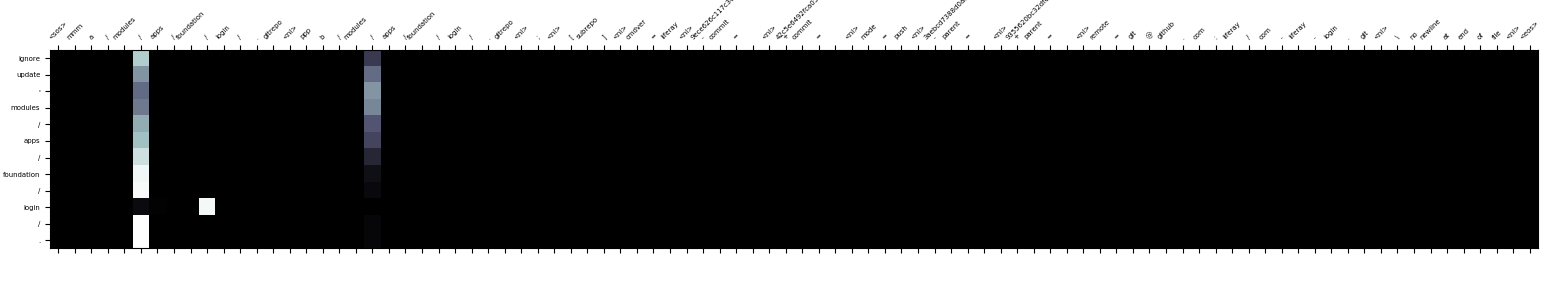
\includegraphics[width=\textwidth]{figs/ignore_attention.png}
        \caption{Attention visualised for a sentence that has the \texttt{ignore update '<filename>'} pattern. The model is able to attend to the specific words in the path name in the diff file to generate the correct label.}
        \label{fig:ignore}
\end{figure}
    
\subsection{Another message from NMT1}\label{app:vis:prepare}
\begin{itemize}
    \item \textbf{True message:} prepared version 0 . 2 - snapshot .
    \item \textbf{Predicted message:} prepare next development version .
\end{itemize}
\begin{figure}[H]
        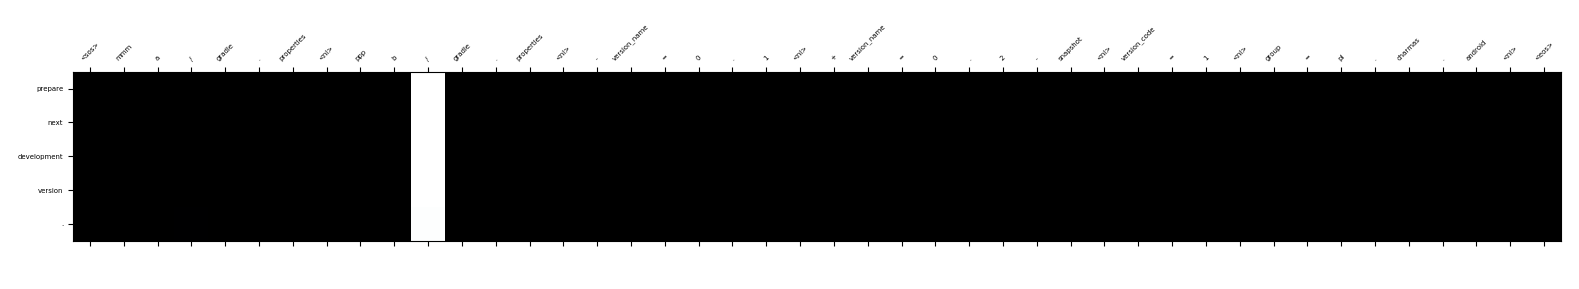
\includegraphics[width=\textwidth]{figs/prepare_attention.png}
        \caption{Attention visualised for a selected example in the testing set. Although the predicted message is close to the real message, the model attends to random parts of the input sequence.}
        \label{fig:prepare}
\end{figure}

\subsection{Distribution of amount of tokens in diffs in the test sets}
\begin{figure}[H]

        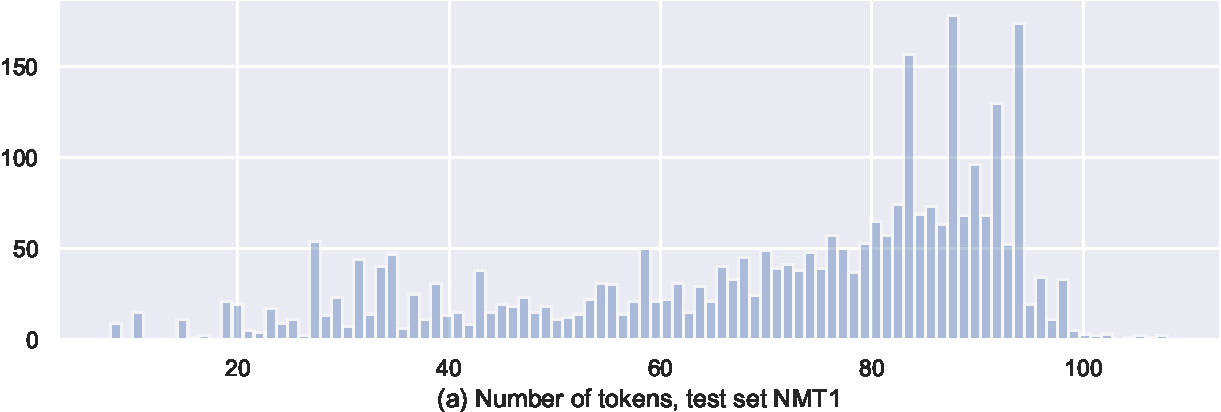
\includegraphics[width=.45\textwidth]{figs/diff_dist_nmt1.pdf}\hfill
        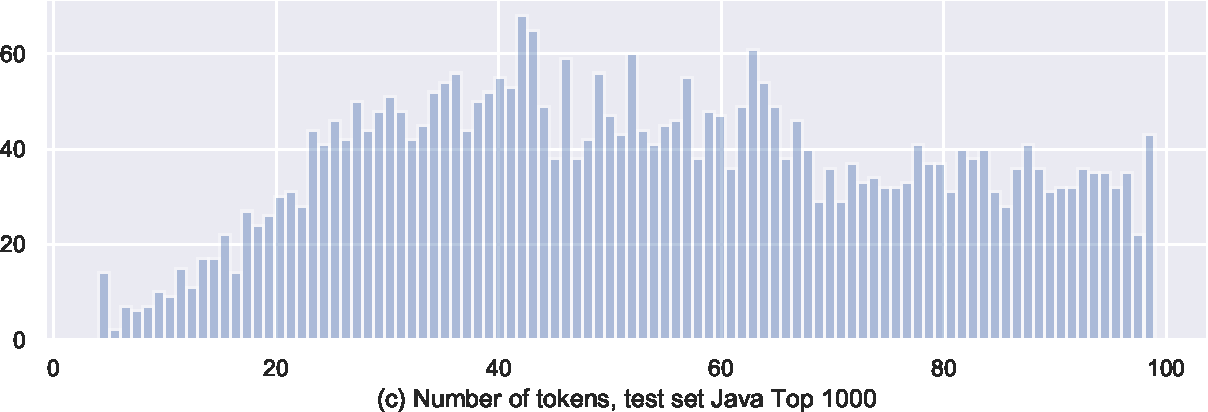
\includegraphics[width=.45\textwidth]{figs/diff_dist_java1000.pdf} \\[.5cm]
    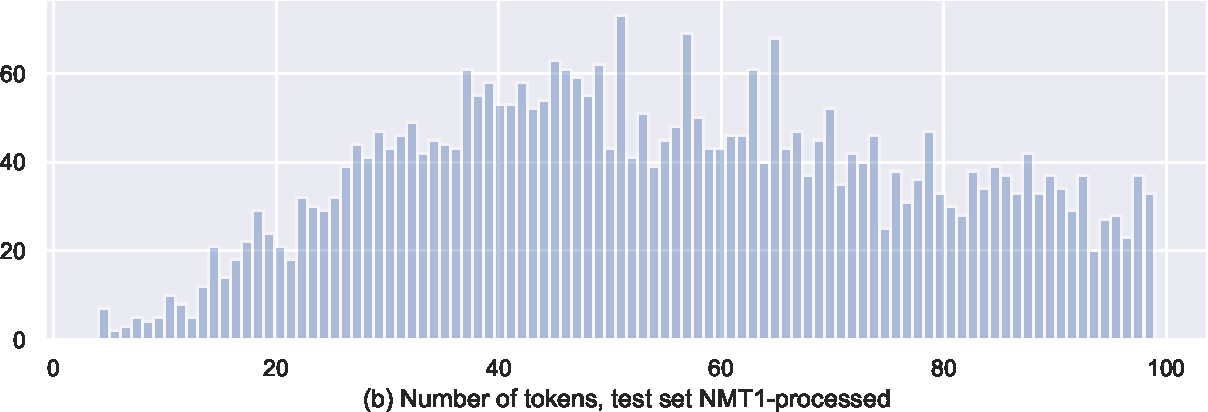
\includegraphics[width=.45\textwidth]{figs/diff_dist_nmt1_proc.pdf}\hfill
    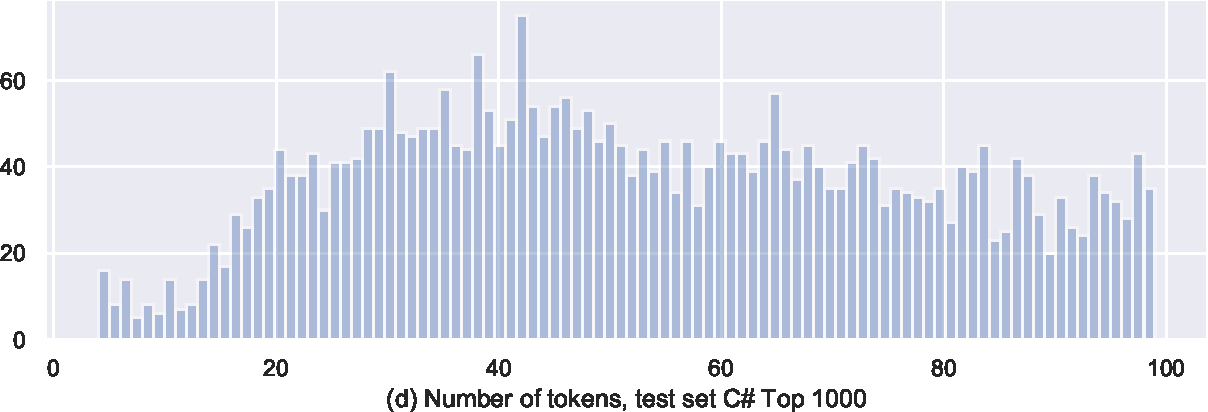
\includegraphics[width=.45\textwidth]{figs/diff_dist_cs1000.pdf}
    \caption{Distribution of amount of tokens in diffs in the test sets}\label{app:vis:tokendist}
\end{figure}